\documentclass[twoside, a4paper, x11names]{article}
\usepackage{amsmath}
\usepackage{float}
\usepackage{graphicx}
\usepackage{url}
\usepackage{etaremune}
\usepackage{listings}
\usepackage{todonotes}
\usepackage{hyperref}
\usepackage[xindy]{glossaries}
\usepackage{fancyvrb}
\usepackage{tikz}
\usetikzlibrary{er}
\makeglossaries
\newfloat{program}{thp}{lop}
\floatname{program}{Listing}
\VerbatimFootnotes
\author{Lukas Hofmaier}
\title{Verifying Type Class Laws with Equational Reasoning}
\newglossaryentry{verification}
{
name=verification,
description={the evaluation of whether a system complies with a specification}
}

\newglossaryentry{referential_transparency}
{
name={referential transparency},
description={an expression is said to be referential transparent if it can be replaced with its value without changing the behavior of a program.}
}

\newglossaryentry{adhoc_polymorphism}
{
name={ad hoc polymorphism},
description={also known as function overloading or operator overloading. Polymorphic functions can be applied to arguments of different types, because a polymorphic function can denote a number of distinct implementations depending on the type of the arguments to which it is applied.}
}

\newglossaryentry{typeclass}
{
name={type class},
description={ a type class is a type system construct that supports ad hoc polymorphism. This is achieved by adding constraints to type variables in parametrically polymorphic types.},
plural={type classes}
}
\newglossaryentry{typesignature}
{
name={type signature declaration},
description={a type signature declaration tells, what type a Haskell variable has.},
plural={type signature declarations}
}

\newglossaryentry{monoid}
{
name={monoid},
description={a monoid is an algebraic structure with single associatve binary operation. they are semigroups with identity.}
}

\newglossaryentry{function-definition}
{
name={function definition},
description={ In Haskell a function definition is an equation. The left-hand side is the function name and it's arguments. The right-hand side is contains the expression of the function body.},
plural={function definitions}
}

\newglossaryentry{associativity}
{
name={associativity},
description={Within an expression containing two or more occurrences in a row of the same associative operator, the order in which the operations are performed does not matter as long as the sequence of the operands is not changed. That is, rearranging the parentheses in such an expression will not change its value.}
}


\begin{document}

\maketitle
%%\tableofcontents

\begin{abstract}

One of the appeals of a purely functional programming language, like Haskell, is that it is substantially easier to verify the correctness of a program. The reason is referential transparency. The fact that function definitions in Haskell are equalities, allows us to reason about properties of a program by substituting expressions with equal expressions. This process is called equational reasoning.

Some type classes in Haskell exhibit properties, the so called “type class laws”, that every corresponding type class instance is expected to obey. These properties ensure certain desirable behavior (e.g. associativity), or they can be used to conclude further properties. Type class laws aren't enforced by the Haskell compiler, so we need to check them ourselfs.
 
This report describes the technique equational reasoning and how it can be used to prove that a type class implementation obeys the corresponding type class laws. Further, it gives a brief description of the concept of a type class and describes the type class \verb|Monoid| and its laws in more detail.
Finally, we walk through an application example. We use equational reasoning to proof a type class law for a simple plugin system written in Haskell. 
\end{abstract}

\section{Introduction}
\label{sec:This}

One of the advantages often claimed by pure functional programming languages is that they are great for \gls{verification} and \emph{equational reasoning} \cite{Wadler87}.
When I started learning to program in a functional language I didn't know precisely what equational reasoning is and how it can be used to verify certain \emph{properties} of a program. I also didn't know what kind of properties of a program can be verified with equational reasoning. In order to grasp equational reasoning I wrote this article.
This article describes the verification method equational reasoning by a practical example. 

\subsection{Why use equational reasoning?}

Equational reasoning can be used as a formal method for software verification. It's a way to proof the correctness of a program. Correctness means that specified properties of the program hold for an arbitrary input. 

A property of a program can be specified in the form of an equation. For example the following equation states a property of the function \verb|fmap|  \footnote{The function \verb|fmap| takes a function \verb|a -> b| as it's first parameter and a container that contains elements of type \verb|a|. It returns a container with elements of type \verb|b|. This is called \emph{mapping}. The type of \verb|fmap| is \verb|(a -> b) -> a -> b|.}.
\begin{equation}
  \label{eq:firstfunctorlaw}
\text{fmap } \text{id}  =  \text{id}  
\end{equation}
 The function \verb|id| is the identity function. The property represented by equation \ref{eq:firstfunctorlaw} says that applying the function \verb|fmap| with the arguments \verb|id| and an arbritrary container is the same as applying the function \verb|id| on a container. Put it another way, mapping the identity function over every item in a container has no effect. Given a function definition of \verb|fmap|, we can check if this property holds or not using equational reasoning.

The goal of equational reasoning is to provide certainty that a program has particular properties. Proof of required properties contribute to the reliability and robustness of a software. 
For example, the first formally verified micro kernel, seL4 was verified using Haskell and formal verification to ensure proper security functionality and security assurance \cite{Klein09}.
Another example is the streaming library "pipes". The author, Gabriel Gonzales, used equational reasoning to prove the correctness of the library \cite{gonzales13}.

\subsection{Why are functional programming languages great for equational reasoning?}

An equation is a statement that two expressions are equal (e.g. $1 + 3 = 4$). And reasoning is the process of thinking about something in a logical way in order to form a conclusion. The technique of equational reasoning implies that we show correctness by showing that two expression of a program are equal. 

The reason why we can use equational reasoning in functional programming is \gls{referential_transparency}. A piece of code can be replaced by its value; this is true in purely functional languages. The absence of side effects allow us the replace the left-hand side of a definition with the right-hand side and vice verca. For example if you have the following Haskell definition:
\begin{verbatim}
x = 23
\end{verbatim}
That means that any \verb|x| can substituted by \verb|23|.

This isn't possible in programs written in an imperative language because in imperative languages the value of an expression depends on the context of the execution environment. In an imperative language \verb|x = 23| is an assigment, not an equality. The variable \verb|x| is mutable and the value of the expression \verb|x| can change at runtime. Hence, we must not substitute \verb|x| with \verb|23| in your program because arbitrary values could be assigned to the variable \verb|x| in other statements of the program.

The programming language Haskell is a purely functional language, which means that functions do not have side effects. Hence, we can verify Haskell programs using equational reasoning. For this reason all examples in this article are written in Haskell.

\subsection{What properties will we discuss?}

Equational reasoning is used to proof that certain properties of a program hold. If we want to verify a program, we have to define one or more properties in the first place. This properties are part of the program specification. We could define arbritrary properties but this article mainly deals with properties derived from the so called \emph{type class laws}. In Haskell type class laws are exhibited by \glspl{typeclass}. For example, the property formed by equation \ref{eq:firstfunctorlaw} is a type class law of the type class \verb|Functor|(functors are described in appendix, section \ref{sec:functor}).

Type classes are a concept to describe the behavior of a type. 
They are very similar to interfaces. If we want to make a type an instance of a type class, we have to implement the functions given by the \glspl{typesignature} of the type class. Figure \ref{fig:typeclassrelation} illustrates the relation between values, types and type classes in Haskell. A type can be a member of serveral type classes. A type class can contain several types. A value has exacty one type and but several values can be of same type.

An instance of a type class must obey the corresponding type class laws. Laws allow us to make assumptions about the behavior of the program and reason about the code. Properties of existing code allow us to rely on expected behavior and deduce further properties for new code. For example, if the property formed by equation \ref{eq:firstfunctorlaw} holds, we can rest assure that \verb|fmap| only applies the function to the items in the container and does nothing more, like changing the structure. If an implementation of \verb|fmap| would change the structure of the container, it would break the property of equation \ref{eq:firstfunctorlaw}.

Type class laws aren't enforced by Haskell. We need to verify them yourself when implementing a instance. We can verify the correctness of these equations using equational reasoning to prove that the instances we build are sound. 

\tikzset{multi  attribute/.style={attribute ,double  distance=1.5pt}}
\tikzset{derived  attribute/.style={attribute ,dashed}}
\tikzset{total/.style={double  distance=1.5pt}}
\tikzset{every  entity/.style={draw=orange , fill=orange!20}}
\tikzset{every  attribute/.style={draw=MediumPurple1, fill=MediumPurple1!20}}
\tikzset{every  relationship/.style={draw=Chartreuse2, fill=Chartreuse2!20}}

\begin{figure}
\centering
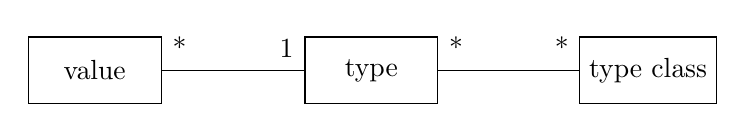
\begin{tikzpicture}[node distance=10em]
  \node[entity](type){type};
  \node[entity](typeclass)[right of=type]{type class};
  \node[entity](value)[left of=type]{value};
  \draw (type) -- (typeclass) node [very near end, above=1pt] {*} node [very near start, above=1pt] {*};
\draw (value) -- (type) node [very near end, above=1pt] {1} node [very near start, above=1pt] {*};
  
\end{tikzpicture}
\caption{Relation between value, type and type class}
\label{fig:typeclassrelation}
\end{figure}
\subsection{Overview}

This article will illustrate in detail how equational reasoning works in practice using the type class laws of the type class \verb|Monoid| as the running example. Section \ref{sec:example} will walk through the process of proofing that an implementation of the \verb|Monoid| type class obeys the first monoid law.  In order understand every step of the process the first three sections will explain the fundamental concepts used in section \ref{sec:example}. The article doesn't require knowledge of type classes and monoids. 
Section \ref{sec:typeclasses} will give a short introduction to type classes with and section \ref{sec:monoid} describes monoids. In section \ref{sec:equationalreasoning} we will give an introduction to equational reasoning in general before we proof the correctnes of the example in section \ref{sec:example}.

This article give answers to the following questions:
\begin{itemize}
\item What are desired properties of your program? Where do the come from? (type classes) Why are they useful? (covered in section \ref{sec:typeclasses})
\item What is equational reasoning? What is the difference between testing and proofing? How do we use equational reasoning to verify properties of a program? (covered in section \ref{sec:equationalreasoning}
\end{itemize}



\section{Type classes}
\label{sec:typeclasses}

This section will give a short description of the concept type class. It will explain the relation to polymorphism and describe type classes \verb|Functor|, \verb|Applicative| and \verb|Monoid| in more detail as these type classes are important for the example in section \ref{sec:example}.

The concept of a type class was introduced as a construct that supports operator overloading and ad-hoc polymorphism \cite{Wadler}.

A type class is like an interface. It contains the function declarations. A type becomes an instance of a type class when it defines all required functions of the type class. When a type is an instance of a type class, we can make certain assumptions about behavior of the type. In contrary to interfaces, type classes aren't types. A value can have the type of an interface but not of a type class.

The concept of a type class is explained by example with the function \verb|show| from the \verb|Prelude|-Library (\verb|Prelude| is a module and part of the standard). \verb|show| converts a given value of a type \verb|a| into a character string. The type of \verb|show| is

\begin{verbatim}
show :: Show a => a -> String
\end{verbatim}

The \verb|Show a| before the \verb|=>| is a type class constraint. \verb|a| is a type variable. A type that has one more type variables is called polymorphic \cite{hutton}. The signature means that \verb|show| takes something that implements the type class \verb|Show| and returns a string. \verb|Show| is a type class. It's possible to call \verb|show| with different types (e.g \verb|show 1|, \verb|show "hello"|). The compiler will lookup the correct definition for us as long the type of the first parameter is an instance of the type class \verb|Show|.  
Any type that implements \verb|Show| can be converted to a character string. Types in this class are \verb|Bool|, \verb|Char|, \verb|Int|, \verb|Float|, \verb|Double| etc.

The type class \verb|Show| is defined as follows:
\begin{verbatim}
class Show a where
    show :: a -> String
\end{verbatim}
The keyword \verb|class| defines a new type class. \verb|a| is the type variable. It represents the type that implements the type class (e.g. \verb|Int| or \verb|Bool|).

Once we have a type class we are able to create instances of that class. The following listing defines a type \verb|Person|. It has fields for name and email address. 
\begin{verbatim}
data Person = Person { name :: String
                       email :: String
                     }
\end{verbatim}

To make \verb|Person| an instance of \verb|Show| we provide a definition for \verb|show :: Person -> String|

\begin{verbatim}
instance Show Person where
    show (Person name _) = name
\end{verbatim}

There many other useful type classes in the standard library.

\begin{description}
\item[Ord] Types with an order relation implement \verb|Ord|.
\item[Eq] For types that can be equated.
\item[Read] Types that can be convertet from a string.
\end{description}

\subsection{Polymorphism and type classes}
\label{sec:polymorphism}
In this section we will describe relation between type classes and polymorhism.
There are two types of polymorphism in Haskell \cite{Cardelli}. Type classes are used for ad hoc polymorhism.
\begin{description}
\item[Parametric polymorphism] Refers to a type that contains type variables. For example the type of the function \verb|id| is 
\begin{verbatim}
id:: a -> a
\end{verbatim}
The \verb|id| function can be used with any type. There are no constraints. At compile time, the type variables are substituted with a concrete type. For example
\verb|Char -> Char|.
\item[Ad-hoc polymorphism] It's a synonym for function overloading or operator overloading. Polymorphic functions can be applied to values with different types. A polymorphic function uses different definitions (implementations) depending on the types of the arguments. If a type can be converted to a string, it can be given the type class \verb|Show|. The type \verb|Person| has to provide an implementation for the function \verb|show|. Applying \verb|show| to \verb|Person| results in a different behavior then applying \verb|show| to an \verb|Int|.
\end{description}

\subsection{Functor}
\label{sec:functor}

Functor is a type class for types, which can be mapped over. 

The type class declaration is shown in Listing \ref{fig:functordeclaration}.
The \verb|f| in the declaration is a type class constructor. Only type constructor can implement \verb|Functor| (\verb|Maybe|, \verb|[]|).

Functor defines all instances must implement the function \verb|fmap|.
\begin{figure}
  \centering
\begin{verbatim}
class Functor f where
    fmap :: (a -> b) -> f a -> f b
\end{verbatim}
  \caption{Functor type class declaration}
  \label{fig:functordeclaration}
\end{figure}

\verb|fmap| takes any function \verb|a -> b| and a value of type \verb|f a| and returns a value of type \verb|f b|. 
If \verb|f| is of type \verb|Maybe| \verb|Int| and the function of type \verb|Int -> String|, \verb|fmap| returns \verb|Maybe String|. 

\verb|fmap| applies a function to a value without altering its structure or context.

Instances of \verb|Functor| are:

\begin{description}
\item[List] \verb|map| for lists for is the same as \verb|fmap|.
\item[Either] \verb|Either e a| is a container. \verb|fmap| applies a function to \verb|a|.
\end{description}

Instances of the \verb|Functor| type class are expected to exhibit certain kinds of properties. This properties are called the functor laws.
The Haskell Compiler doesn't detect violations of the expected laws. All Functor instances in the standard library obey these laws.

A Functor instance has to satisfy the following laws \cite{Marlow_2010}.

\begin{description}
\item[Law 1] Mapping the identity function over a functor value, will not change the functor value. Formally
\begin{verbatim}
fmap id  ==  id
\end{verbatim}
\item[Law 2] The second law states that it doesn't matter if we compose two functions and them map them over a functor or if we first map one function over the functor and then map the other function. Formally
\begin{verbatim}
fmap (g . h) = fmap g . fmap h
\end{verbatim}
This is the same as \verb|fmap (g . h) = fmap g (fmap h)|
\end{description}

If we can prove that a type satisfies these laws, we can make assumptions about how the the type will act. And we know that \verb|fmap| only maps the function over the functor. It will not change the structure or the context of the functor.

If we know, that a type satisfy the laws, we are able to deduce further properties for our own types. All type class instances in the standard library satisfy the laws \cite{yorgey}.

\begin{figure}
  \centering
\begin{verbatim}
fmap id = id
fmap (g . h) = fmap g . fmap h
\end{verbatim}
  \caption{The Functor laws}
  \label{fig:functorlaws}
\end{figure}

\subsection{Applicative Functor}
\label{sec:applicatives}

Applicative functors are an abstract characterisation of an applicative style of effectful programming \cite{mcbride} \cite{control.applicative}

The \verb|Applicative| type class encapsulates the following idea. What if you have a function wrapped in a \verb|Functor| (e.g \verb|Maybe (Int -> Int -> Int)|) and you want to apply the function to another functor. 

The \verb|Applicative| type class is defined as follows.
\begin{verbatim}
class (Functor f) => Applicative f where
    pure :: a -> f a
    (<*>) :: f (a -> b) -> f a -> f b
\end{verbatim}

Applicatives are enhanced functors. They are able to map a function encapsulatet in a functor over another functor.

\begin{figure}
  \centering
     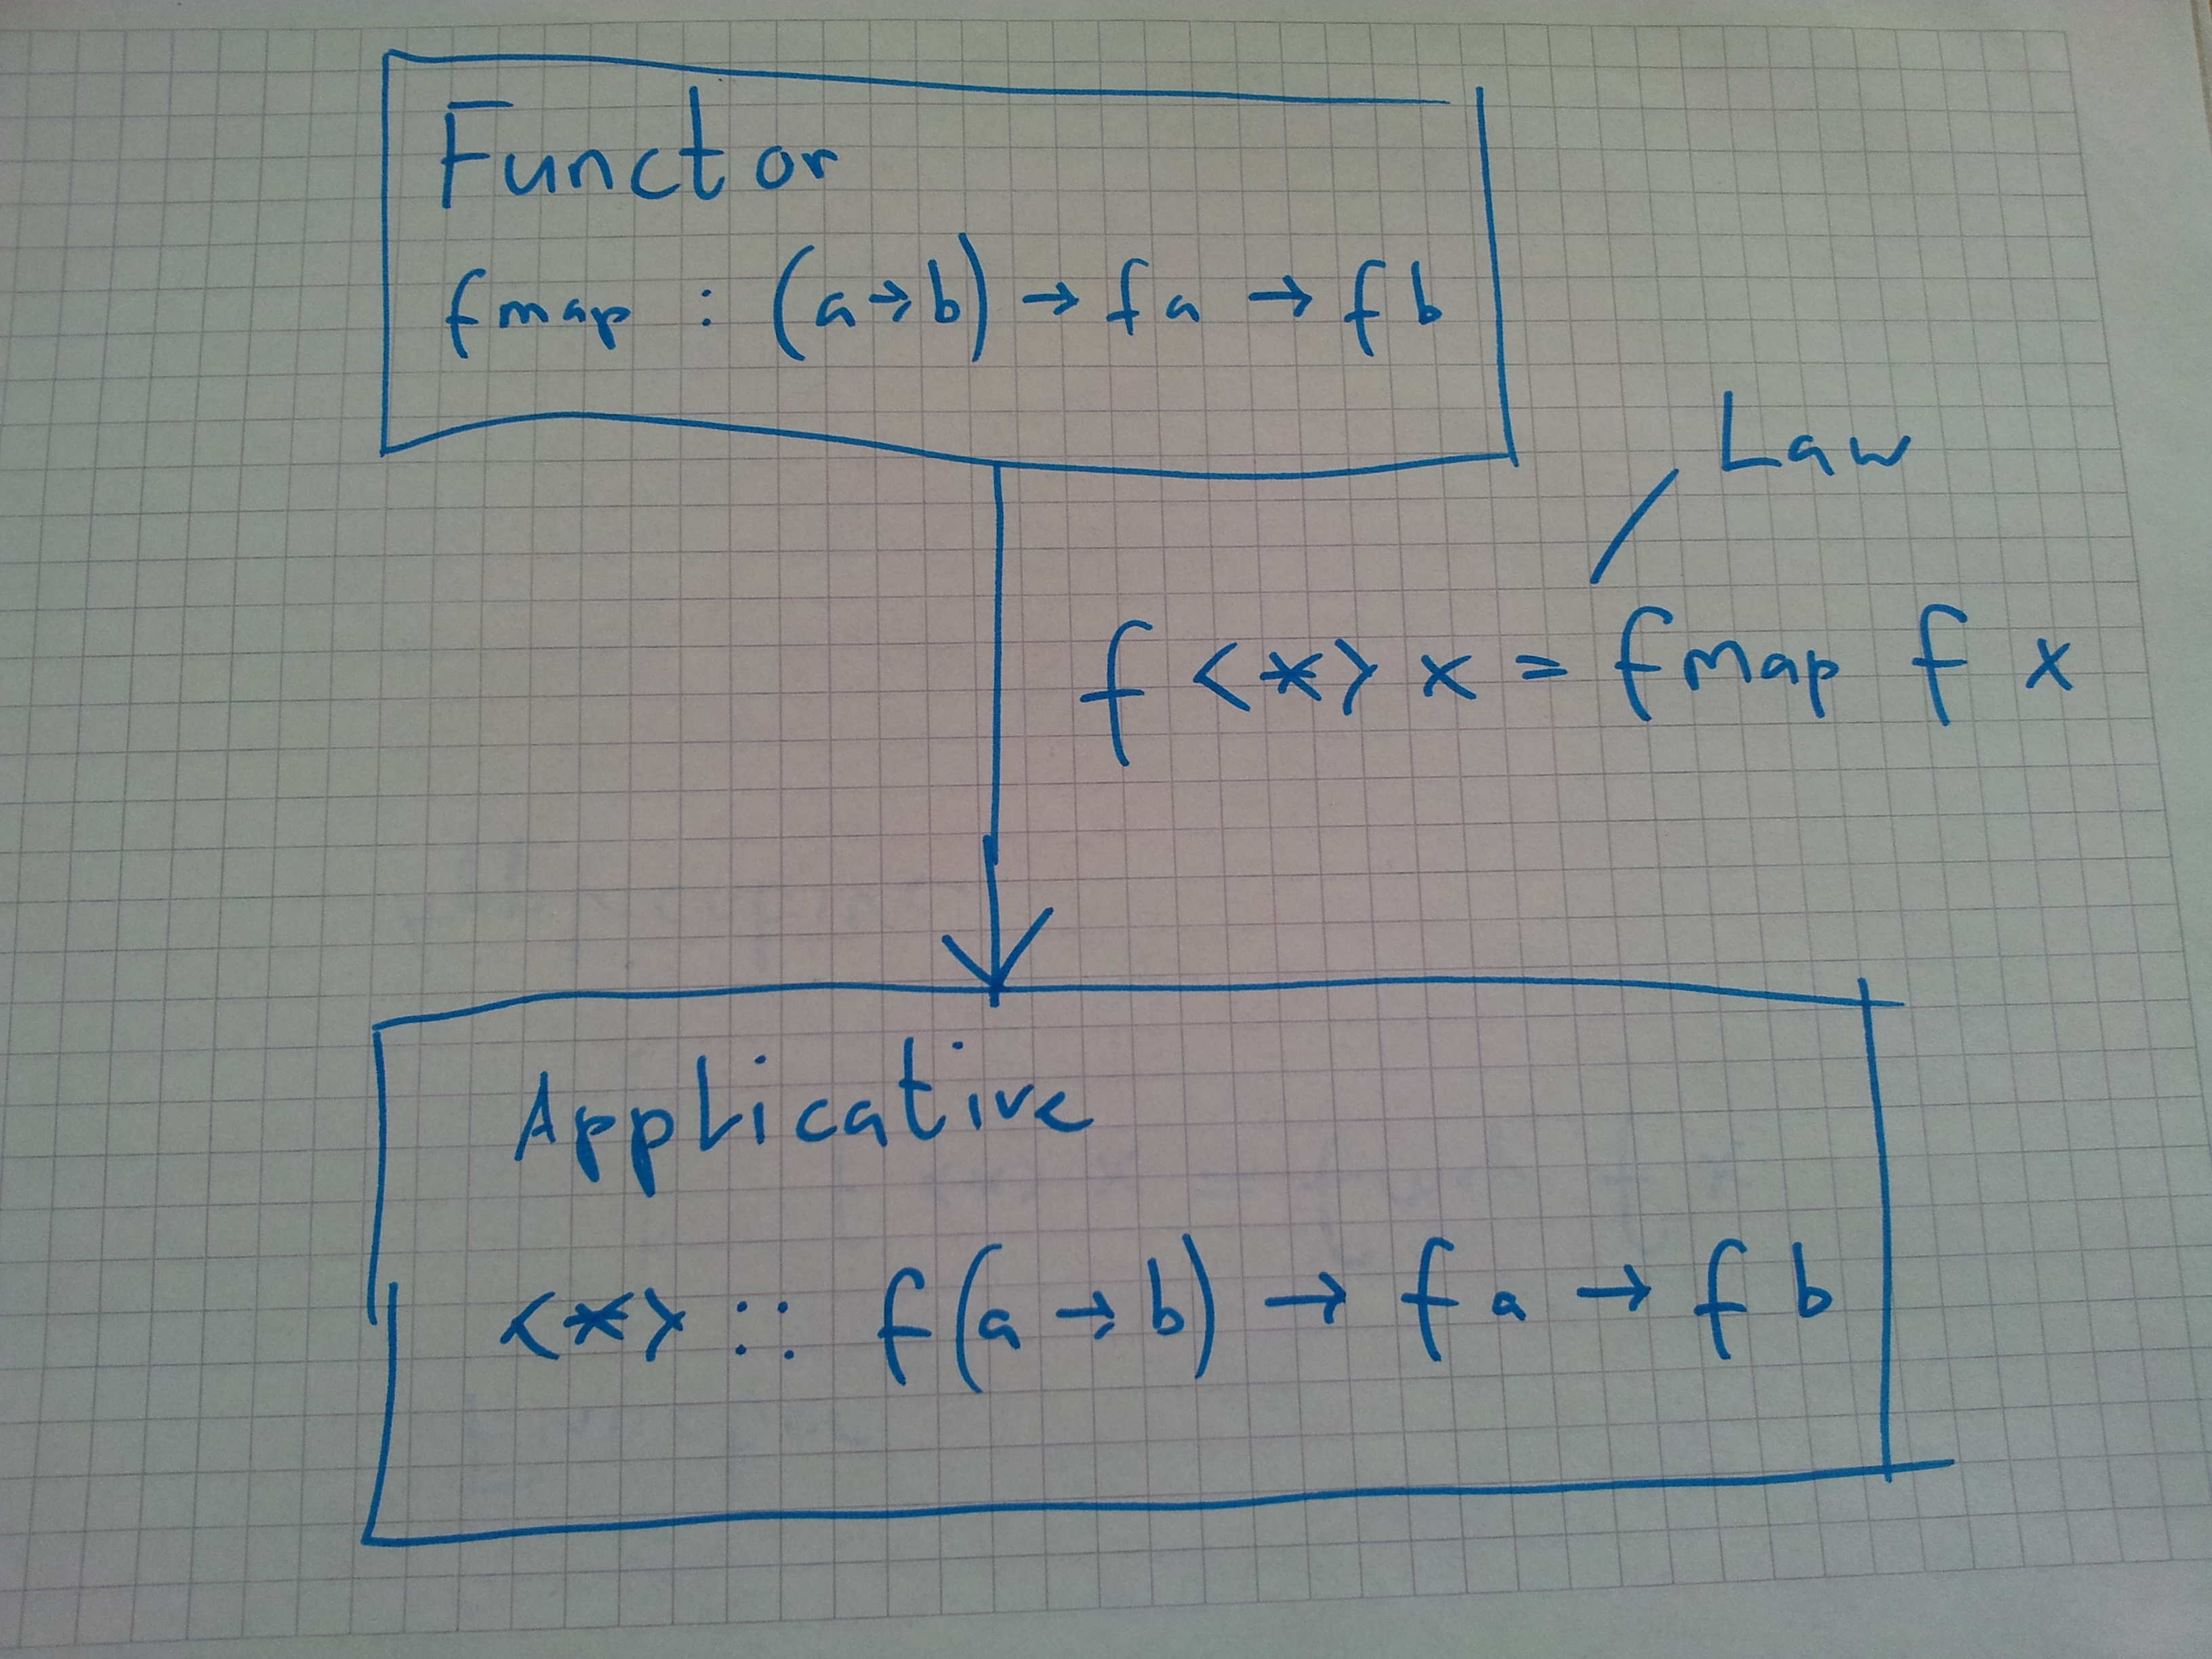
\includegraphics[width=0.9\textwidth]{functor_applicative}
  \caption{Comparison of test, property-based-testing and proof}
  \label{fig:property_validation}
\end{figure}


The following type are instances of the type class \verb|Applicative|

\begin{itemize}
\item Maybe
\item IO
\end{itemize}

\subsection{Monoid}
\label{sec:monoid}

Some types, let's say \verb|a|, have a binary function with the type declaration. 
\begin{verbatim}
f :: a -> a -> a
\end{verbatim}

The type \verb|a| has a value that serves as identity for the given function. For example 1 is the identity for the multiplication. Multiplicaiton with an other numer $x$ results always in $x$.

Several value of type \verb|a| can always be reduces to a single value. It doesn't matter in which order we apply the function, the result is always the same. This is called associativity.

If type \verb|a| has this behavior, it's a monoid and it can be an instance of the \verb|Monoid| type class.

The \verb|Monoid| type class is define as follows:
\begin{verbatim}
class Monoid m where
    mempty :: m
    mappend :: m -> m -> m
    mconcat :: [m] -> m
    mconcat = foldr mappend mempty
\end{verbatim}

The \verb|Monoid| type class is define in \verb|Data.Monoid| \cite{monoid}. 

From the type class definition we see that concrete type can be made instances of \verb|Monoid|. 

\verb|mempty| return the identity value. The binary function is \verb|mappend|. It takes to values of the same type and returns another value of that type. \verb|mconcat| takes a list of monoids and reduces them \verb|mappend| to a single value, applying mappend. It has a default implementation.

When making monoid instances, we need to make sure that \verb|mempty| acts like the identity with respect to the \verb|mappend| function and \verb|mappend| must be assocative. There are three monoid laws

\begin{enumerate}
\item \verb|mappend mempty x = x|
\item \verb|mappend x mempty = x|
\item \verb|(x `mappend y) `mappend z = x `mappend (y `mappend z)|
\end{enumerate}

The following Haskell types are \verb|Monoid| instances
\begin{description}
\item[List] The empty list \verb|[]| and \verb|++| (concatenation) form a monoid.
\item[Product and Sum] Numbers can be monoid with respect to multiplication or addidion. There are two monoid instances for \verb|Num|.
\item[Maybe] Can also be an instance of \verb|Monoid|.
\end{description}

An interesting property of the \verb|Applicative| type class with respect to the monoid type class is, if \verb|f| is an \verb|Applicative| and \verb|m| is a \verb|Monoid|, \verb|f b| is also a \verb|Monoid|. This is because we can make an \verb|Applicative| with the given property an instance of \verb|Monoid|.
\begin{program}
\begin{verbatim}
instance (Applicative f, Monoid b) => Monoid (f b) where
    mempty = pure mempty

    mappend = liftA2 mappend
\end{verbatim}
\label{lst:applicative2monoid}
\caption{Applicative property}
\end{program}

As \verb|f| is an applicative, it implements \verb|pure|. The \verb|mempty| function returns the identity value of \verb|b| in a default context. \verb|liftA2| encapsulates the \verb|mappend| function in a applicative functor. It's possible to prove this property with equational reasoning.

\section{Equational Reasoning}
\label{sec:equationalreasoning}

Verification is the process of checking if software does what it's specification demands. To verify a program, a specification is required. In the case of functions that implement an instance of the type classes of section \ref{sec:typeclasses}, the specification is defined in form of the type class laws.
This section will compare different verification techniques and describe the method equational reasoning by example using type class laws as specification. In section \ref{sec:example} equational reasoning will be applied to proof the property of listing \ref{lst:monoidinstance1} in section \ref{sec:typeclasses}.

There are several ways to check the behavior of a program. 
We will describe the difference with a simple example. Given the following property:

\begin{equation}
  \label{eq:reverse_prop}
\text{reverse} (\text{reverse } xs) = xs  
\end{equation}
Equation \ref{eq:reverse_prop} expresses, if we apply \verb|reverse| twice on the same list \verb|xs| we get back the original list \verb|xs|. \verb|reverse| is the inverse of \verb|reverse| (other functions, like \verb|id|, have this property too). Verification techniques allow us to check if equation \ref{eq:reverse_prop} holds. We describe three techniques. The first two, testing and property-based testing, are very common and the third is the topic of this article.

\begin{description}
\item[Testing] Run the program with a selected input and check if it behaves as expected. In order to check the behavior, a function evaluates both sides of the equation \ref{eq:reverse_prop} and compares the values. The following listing shows an example test.

\begin{lstlisting}[caption={Function definition for testing},label={lst:testing}]
input = [1,2,3]

test_reverse :: [Int] -> Bool
test_reverse xs = reverse (reverse xs) == xs
\end{lstlisting}

The selected input is \verb|[1,2,3]|. \verb|test_reverse| evaluates to a Boolean expression to indicate if the property holds for the given input. It's necessary to run the program to evaluate \verb|test_reverse|.
An advantage of this method is, that the programmer doesn't have to define general properties. The specification is expressed with a concrete input value and a concrete output value. It's easier to think about a concrete input and the corresponding output value than to find general properties that a function must obey.
\item[Property-based testing] The input for the test program is generated randomly. The tests are executed by a tool (e.g. Quickcheck).
\item[Proof] A Proof can show that a property holds in all circumstances. To prove a property we use the technique equational reasoning. This technique requires knowledge of the function definition.
\end{description}

Figure \ref{fig:property_validation} compares the input coverage of the described methods. Testing checks if the program behaves correctly with one chosen point of the input space. Property-based testing checks the behavior at hundreds of randomly-generated points. Proof covers all possible cases of the possible input. It is the most reliable verification.

\begin{figure}
  \centering
     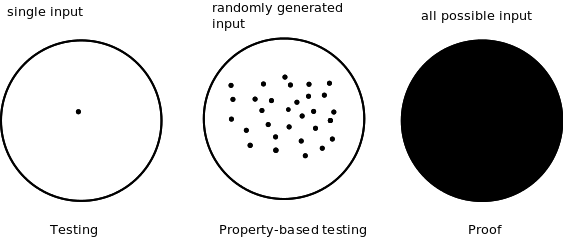
\includegraphics[width=0.9\textwidth]{testing}
  \caption{Comparison of testing, property-based-testing and proof}
  \label{fig:property_validation}
\end{figure}

\subsection{Reasoning about algebraic properties}

Equational reasoning is a method originally used in algebra. It's the process of proving a given property by substituting equal expressions.
For example, it's possible to show that the following property holds:
\begin{equation}
  \label{eq:sum}
  (x+a)(x+b) = x^2 + (a+b)x+ab
\end{equation}
To show that the equality holds, we have to transform the expression on the left-hand side  $(x+a)(x+b)$  to an equal expression on the right-hand side with the help of the basic algebraic properties of numbers (distributivity, commutative, associative, ) until we get $x^2 + (a+b)x+ab$  \cite{hutton}. 

In the first step (equation \ref{eq:firstalgebra} we use distributivity to expand the term on the left-hand side.
\begin{equation}
  \label{eq:firstalgebra}
  (x+a)(x+b) = x^2 + ax + xb + ab \text{     (use distributivity)}
\end{equation}
In the second step we use commutativity to substitute $xb$ with $bx$.
\begin{equation}
x^2 + ax + xb + ab = x^2 + ax + bx + ab \text{     (use commutativity)}
\end{equation}
In the last step we use distributivity to factorize $x$ and we get $x^2 + (a+b)x+ab$.
\begin{equation}
x^2 + ax + bx + ab = x^2 + (a + b)x + ab \text{     (use distributivity)}
\end{equation}
All we did, was substituting expression according the algebraic properties 

\subsection{Reasoning about Haskell programs}

A function definition in Haskell means that we can substitute the left-hand side with the right-hand side and vice versa. This is possible because Haskell is a purely functional language. Hence, we can use the same approach to prove that a property of a program written in Haskell holds, as we used to reason about mathematical expressions. 
For example, it's possible to show that the length of a list with one element is actually 1. This general property can be formed as boolean expression in Haskell.
\begin{verbatim}
length [x] == 1
\end{verbatim}
The property holds no matter what \verb|x| is. To show that, we use the \gls{function-definition} of \verb|length| as a general description of the behavior. Listing \ref{lst:lengthdefinition} shows the definition of \verb|length| \cite{hutton}.
\begin{lstlisting}[caption={Function definition of length},label={lst:lengthdefinition}]
length [] = 0
length (x:xs) = 1 + length xs  
\end{lstlisting}

To conclude that \verb|length [x] == 1| is always true, we substitute \verb|length [x]| until we get \verb|1|. Listing \ref{lst:lengthproof} shows the step by step substitution.
\begin{lstlisting}[caption={Deduce that the length of a list with one element is 1},label={lst:lengthproof}]
length [x] = 
length (x:[])   -- [x] is the same as x:[]
1 + length []   -- apply definition
1 + 0           -- apply defintion
1               -- 1 + 0 = 0
\end{lstlisting}
Function definitions are general description and we can use them to deduce other general properties by substituting equal expressions.

\subsection{Proof by structural induction}
\label{sec:induction}

If we apply simple substitution to a recursive function, we run into problems.
Consider the \gls{function-definition} of \verb|length| in listing \ref{lst:lengthdefinition}.
If we substitute \verb|length x| with the definition \verb|1 + length xs|, we end up substituting \verb|length x| forever. A way to verify recursive programs is to use proof by structural induction.  
Structural induction for proofing a property can be used for list or algebraic data types with a recursive constructor (e.g. Tree).

 The principle of induction states, that it is sufficient to prove a property $p$ for the base case and that $p$ is preserved by the inductive case. In order to prove $p$, two steps are required:
 \begin{description}
 \item[Base case] Prove $p(0)$ is true.
 \item[Induction step] Prove $p(n+1)$ if $p(n)$ (induction hypothesis) is true.
 \end{description}

Proof by induction is similar to writing a recursive function. Recursive functions use a base case (e.g. \verb|[]|, 0). 
If we use structural induction we proof the base case. We show that the property holds for a concrete input value (e.g. \verb|[]|, 0). 

In a recursive function definition we define \verb|f (x:xs)| and use \verb|f x| in the right-hand side. In the proof we show that $p(n+1)$ with the assumption $p(n)$.

We explain proof by structural induction with another example. We verify that the overall length of two concatenated lists $xs$ and $ys$, is the same as the sum of the length of $xs$ and the length of $ys$.  The ++-operator concatenates two lists.
\begin{equation}
  \label{eq:lengthprop}
  \text{length (xs ++ ys)} = \text{(length xs) + (length ys)}
\end{equation}
In order to verify property \ref{eq:lengthprop}, we need the function definitions for \verb|length| and \verb|(++)|.
The Prelude functions \verb|length| and \verb|(++)| are given in listing \ref{lst:lengthdefinition} and \ref{lst:concatdefintion}.

\begin{lstlisting}[caption={Haskell function definition of the concatenation operator},label={lst:concatdefintion}]
[] ++ xs = xs
(x:xs) ++ ys = x:(xs++ys)
\end{lstlisting}

\begin{description}
\item[Base case]
We have to show that property \ref{eq:lengthprop} holds for the base case. The base case, in this example, are the arguments \verb|[]| and an arbitrary list for \verb|ys|. It isn't necessary to replace \verb|ys| because the definition of \verb|++| uses recursion over \verb|xs|. \verb|ys| will always be the same list.
In order to check if property \ref{eq:lengthprop} holds for the base case, we replace \verb|xs| with  \verb|[]|, leading to

\begin{verbatim}
length ([] ++ ys) == length [] + length ys
\end{verbatim}

We will evaluate the expression on the left-hand side and the right and side separately.
The left-hand side evaluates to

\begin{verbatim}
length ([] ++ ys) -- apply ++
length ys
\end{verbatim}

The right-hand side evaluates to 

\begin{verbatim}
length [] + length ys     -- apply length []
0 + length ys
length ys
\end{verbatim}

When we evaluate each side of the equation \ref{eq:lengthprop} with the value \verb|[]| for \verb|xs|, the result is \verb|length ys| on both sides. Hence, property \ref{eq:lengthprop} holds for the base case.

\item[Induction step]
 We have to prove that the two expressions on both sides of the \verb|=| sign in listing \ref{lst:inductionstep} are equal
\begin{lstlisting}[caption={The left-hand side and the right-hand side have to be equal},label={lst:inductionstep}]
length ((x:xs) ++ ys) = length (x:xs) + (length ys)
\end{lstlisting}

with the assumption (induction hypothesis).
\begin{equation}
  \label{eq:induction_hypothesis}
      \text{length(xs ++ ys)} = \text{length(xs) + length(ys)}
\end{equation}

Again, we evaluate the the left-hand side of equation in listing \ref{lst:inductionstep}.

\begin{program}
\begin{verbatim}
length ((x:xs) ++ ys)     --apply definition of ++
length (x:(xs ++ ys))      --apply definition of length
1 + length (xs ++ ys)      --use induction hypothesis
1 + length xs + length ys
\end{verbatim}
\end{program}

If we evaluate the right-hand side of the equation in listing \ref{lst:inductionstep} we get:
\begin{program}
\begin{verbatim}
length (x:xs) + length ys    -- apply definition of length
1 + length xs + length ys
\end{verbatim}
\end{program}

The last listing shows, that the equality in listing \ref{lst:inductionstep} follows from the induction hypothesis in equation \ref{eq:induction_hypothesis}. This completes the induction step and therefore the proof itself.
\end{description}

The previous example used \glspl{function-definition} of \verb|length| and \verb|(++)|. In order to apply equational reasoning we have to know the function definitions of involved functions or we can rely on already proven properties. 
For example all types of the standard library, that are an instance of a type class, satisfy the type class laws (see \ref{sec:typeclasses}) \cite{yorgey}. Some libraries exhibit properties in their documentation (e.g. pipes library \cite{gonzales13}). 
\section{Example proof for Monoid Laws}
\label{sec:example}
In this example we use equational reasoning (see section \ref{sec:equationalreasoning}) to prove the monoid laws (see section \ref{sec:monoid}) for a new type.
The following example is taken from a blog post of Gabriel Gonzales \cite{gonzales14}. 

Suppose we want to build a plugin system. A plugin in our example is a \verb|IO| action, that takes a \verb|Char| value and does some work with it (e.g. log to a file, potentially with side effect). We demand the following requirements:
\begin{itemize}
\item We want to be able to add an arbitrary number of plugins.
\item The plugins should be composable.
\item The order we add the plugins must not matter.
\end{itemize}

A monoid instance satisfies all listed requirements. We could use the \verb|mappend| operator to compose several plugins. Hence, if we can prove that the plugins satisfy the monoid laws, we can combine them, using the monoid function \verb|mappend| and we are able to add plugins without concerning about the order of evaluation. In addition they are easier to use because, they will behave as expected.

The following listing shows the use of a plugin. The \verb|logto| function is a plugin. The program will read a character \verb|c| from the command line and apply the given plugin to \verb|c|.

\begin{verbatim}
main = do
    handleChar <- logto
    c <- getChar
    handleChar c
\end{verbatim}

To append additional plugins, e.g. \verb|print2stdout|, we compose a new monoid with the \verb|mappend| function.
\begin{verbatim}
handleChar <- mappend logto print2stdout
\end{verbatim}
The definition of \verb|logTo| is shown in the following listing: 

\begin{verbatim}
logTo :: IO ( Char -> IO ())
logTo = do
    handle <- openFile "log.txt" WriteMode
    return (hPutChar handle)
\end{verbatim}

The plugins are of type \verb|IO ( Char -> IO ())|. Hence we have to provide a monoid instance implementation for the type \verb|IO ( Char -> IO ())|. Instead of writing a specialized instance for \verb|IO ( Char -> IO ())|, we use the general implementation of section \ref{sec:monoid}.
The instance implementation is repeated for convenience:

\begin{lstlisting}[caption={Monoid instance},label={lst:monoidinstance}]
instance (Applicative f, Monoid b) => Monoid (f b) where
    mempty = pure mempty

    mappend = liftA2 mappend
\end{lstlisting}
The generalization has the advantage, that we have to prove the type class law only once for all types that match the general type declaration. The process of verifying a program is cumbersome and time consuming. Generalization of proofs is desirable.

We will first describe, why the instance implementation of listing \ref{lst:monoidinstance} makes the type \verb|IO ( Char -> IO ())| part of the \verb|Monoid| type class. Then we prove that the monoid laws from section \ref{sec:monoid} hold for the definition in listing \ref{lst:monoidinstance}. We will assume that the instance implementation of listing \ref{lst:monoidinstance} is a monoid in the first part.

\subsection{Generalization of the plugin type }
\label{sec:generalization}

In order to use the instance implementation of listing \ref{lst:monoidinstance} the type \verb|IO| has to be part of the type class \verb|Applicative| and the type \verb|Char -> IO ()| has to be a \verb|Monoid|. 
Hence we have to check if \verb|Char -> IO ()| is a monoid. We use the instance definition of listing \ref{lst:monoidinstance} again and say: \verb|Char -> IO ()| is a monoid if the type \verb|(->) Char| (that's the type of a haskell function) is part of the \verb|Applicative| type class and the type \verb|IO ()| is a monoid. We repeat the same argument for \verb|IO ()|.

Here is an overview of all the steps of the argumentation:
\begin{enumerate}
\item show that  \verb|IO ( Char -> IO ())| is of type 
\begin{verbatim}
(Applicative f, Monoid b) => Monoid (f b)
\end{verbatim}
\item show that \verb|Char -> IO ()| is a monoid
\item show that \verb|IO ()| is a monoid
\item show that \verb|()| is a monoid
\end{enumerate}

We show the required properties in reversed order.

\begin{etaremune}
\item The standard library provides a monoid instance for \verb|()| \cite{monoid}. In this article we will believe the fairy tale of abstraction and assume that the implementation of the standard library satisfies the monoid laws.
\item \verb|IO ()| is a monoid, because \verb|IO| is part of the \verb|Applicative| type class \cite{control.applicative} and \verb|()| is a monoid if the implementation from listing \ref{lst:monoidinstance} satisfies the monoid laws.
\item The type \verb|(->) r| (that's the type of haskell functions) is a part of the \verb|Applicative| type class \cite{control.applicative}.
 \verb|Char -> IO ()| is a monoid because \verb|(->) Char| is a applicative and \verb|IO ()| is a monoid if the implementation from listing \ref{lst:monoidinstance} satisfies the monoid laws.
\item The compiler will use the instance implementation for \verb|Monoid| type class from listing \ref{lst:monoidinstance} for the type \verb|IO (Char -> IO ())| because it matches the type
\begin{verbatim}
(Applicative f, Monoid b) => Monoid (f b)
\end{verbatim}

\end{etaremune} 

Notice that we rely heavily on the assumption that listing \ref{lst:monoidinstance} satisfies the monoid laws. The next section will prove that the implementation is correct.

\subsection{Proof}
\label{sec:exampleproof}

In this section we will show that the implementation in listing \ref{lst:monoidinstance} satisfies the left identity law of the \verb|Monoid| type class (see section \ref{sec:monoid}).
The left identity law demands that:
\begin{verbatim}
mappend mempty x = x
\end{verbatim}

We will use equational reasoning (see section \ref{sec:equationalreasoning}) to show that the left-hand side is equal to \verb|x|. First we will use the definitions of \verb|mappend| and \verb|mempty| of listing \ref{sec:equationalreasoning} to substitute the left-hand side. Furthermore we look-up the definition of \verb|liftA2| in the source code \cite{control.applicative} to evaluate the expression. 
\verb|liftA2| is defined as follows
\begin{verbatim}
liftA2 f x y = (pure f <*> x) <*> y
\end{verbatim}

\begin{verbatim}
mappend mempty x                           -- def. mappend
= liftA2 mappend mempty x                  -- def. mempty
= liftA2 mappend (pure mempty) x           -- def. liftA2
= (pure mappend <*> pure mempty) <*> x
\end{verbatim}

To resolve this expression further, we use the laws described in section \ref{sec:applicatives}.
One law of the \verb|Applicative| type class says:
\begin{verbatim}
pure f <*> pure x = pure (f x)
\end{verbatim}
We can use this property substitute the left-hand side. Next we write \verb|mappend mempty| as lambda function \verb|\a -> mappend mempty a| and use the monoid law
\begin{verbatim}
mappend mempty x = x
\end{verbatim}
to simplify the expression. In the last step we use the first applicative law
\begin{verbatim}
pure id <*> v = v
\end{verbatim}
 to rewrite the expression as \verb|x|.
\begin{verbatim}
(pure mappend <*> pure mempty) <*> x    -- 3. applicative law
= pure (mappend mempty) <*> x           -- transform to lambda
= pure (\a -> mappend mempty a) <*> x   -- 1. monoid law 
= pure (\a -> a) <*> x                  -- a -> a = id
= pure id <*> x                         -- 1. applicative law
x
\end{verbatim}

That completes the proof.
\todo{right identity und associativity beweisen. Die Beweise brauchen mehrere Seiten und erklaeren nichts neues. Weglassen oder Appendix?}

The example demonstrated several ideas:
\begin{itemize}
\item Type classes allow us to generalize definitions. A prove for the generalization is valid for all specializations.
\item To prove a type class law we can use equational reasoning.
\item Type class laws (or properties) allow to prove further properties.
\end{itemize}



\section{Conclusion}

This article illustrated the verification method equational reasoning by example. We proved that the monoid law, left identity, holds for a given function definition. 

The type class laws provide a specification for the verification process. In addition, we can rely on properties of existing type class instances to prove further properties.

Type classes allow us to generalize definitions. A prove for the generalization is valid for all specializations. Hence, the proof is reusable.

The examination of the topic improved my comprehension for the advantages of a purely functional language. The reason why verification in a purely functional language like Haskell is easier, is because functions are just equalities. We can reason about Haskell code in the same way we reason about mathematical equations. The definitions are stateless. This fact doesn't apply to mainstream languages. A function definition of an imperative language is allowed to change the context. These definitions are stateful.

Personally, I found the process of proving the left identity law for the given definition tedious and demanding. The proof requires creativity and a strong mathematical background. The verification process would be too cumbersome and expensive to apply it to every piece of software. Alltough equational reasoning  isn't suitable for software with a short lifecycle, I think that it's important to know the difference between testing and verification by proof.


\section{Appendix}
\label{sec:appendix}

\subsection{Functor}
\label{sec:functor}

Functor is a type class for types, which can be mapped over. Another way to describe functors is that they represent some sort of computational context \cite{yorgey}. The general concept of a functor is more abstract and harder to grasp than the concepts of type classes described in section \ref{sec:typeclass}.
The most accurate way to describe the type class \verb|Functor| is to give it's declaration \cite{data.functor}:

\begin{verbatim}
class Functor f where
    fmap :: (a -> b) -> f a -> f b
\end{verbatim}

The \verb|f| in the declaration is a type class constructor. Only type constructor can implement \verb|Functor| (e.g. \verb|Maybe|, \verb|[]|).

\verb|fmap| takes any function \verb|a -> b| and a value of type \verb|f a| (\verb|f| is the container or context, \verb|a| is the type wrapped inside the functor) and returns a value of type \verb|f b|. 
If \verb|f a| is of type \verb|Maybe| \verb|Int| and the function of type \verb|Int -> String|, \verb|fmap| returns \verb|Maybe String|. 

Examples of \verb|Functor| instances are:

\begin{description}
\item[List] \verb|fmap| applies the function to every element in the list.
\item[Either] \verb|Either e a| is a container. \verb|fmap| applies a function to \verb|a|.
\end{description}

To make a type an instance of \verb|Functor|, it has to define \verb|fmap|. In addition, the instances are expected to exhibit certain properties. The declaration of the type class doesn't reveal these properties. They are described in the type class documentation \cite{data.functor} \cite{Marlow_2010}. These properties are called the functor laws.
The Haskell Compiler doesn't detect violations of the expected laws. All Functor instances in the standard library obey these laws \cite{yorgey} \cite{Lipovaca}.

A \verb|Functor| instance has to satisfy the following laws.

\begin{description}
\item[Law 1] Mapping the identity function over a \verb|Functor| value, will not change the functor value. Formally
\begin{verbatim}
fmap id  ==  id
\end{verbatim}
\item[Law 2] It doesn't matter if we compose two functions and then map them over a functor or if we first map one function over the functor and then map the other function. Formally
\begin{verbatim}
fmap (g . h) = fmap g . fmap h
\end{verbatim}
This is the same as \verb|fmap (g . h) = fmap g (fmap h)|
\end{description}

If we can prove that a type satisfies these laws, we can make assumptions about how the the type will act. We know that \verb|fmap| will not change the structure or the context of the functor.
And we know that \verb|fmap| only maps the function over the functor and nothing else. 

If we know that a type satisfies the laws, we are able to deduce further properties for our own types. In section we \ref{sec:example} give an example of this process.

\subsection{Applicative Functor}
\label{sec:applicatives}

Applicative functors are abstract characterizations of an applicative style of effectful programming \cite{mcbride} \cite{control.applicative}

The \verb|Applicative| type class encapsulates the following idea. What if you have a function wrapped in a \verb|Functor| (e.g. \verb|Maybe (Int -> Int -> Int)|) and you want to apply the function to another functor (e.g. \verb|Maybe Int|). For example, we want to map \verb|Just (3 *)|, a function encapsulated inside a functor, over \verb|Just 23|, another functor with an encapsulated \verb|Int|. \verb|fmap| doesn't work here, because it expects a function of type \verb|a -> b| as first parameter. That's where the \verb|Applicative| type class comes in. 
The \verb|Applicative| type class is defined as follows \cite{control.applicative}.
\begin{verbatim}
class (Functor f) => Applicative f where
    pure :: a -> f a
    (<*>) :: f (a -> b) -> f a -> f b
\end{verbatim}

The type class declaration demands the type \verb|f| to be a functor. Every type that is part of \verb|Applicative| is part of \verb|Functor|. Hence we can use \verb|fmap| with \verb|Applicative| instances.
Applicatives are enhanced functors. In addition to \verb|fmap| we can use the \verb|<*>| operator to chain several \verb|Applicative| values together.

The \verb|pure| function puts a value of type \verb|a| in a default context. If applied with a function \verb|a -> b|,  \verb|pure| returns a functor with a function inside, \verb|f (a -> b)|, hence the first argument to \verb|<*>|.

It's possible to chain applicatives together as follows:
\begin{verbatim}
ghci> pure (*) <*> Just 3 <*> Just 23
Just 69
\end{verbatim}

The following types are instances of the type class \verb|Applicative|:

\begin{itemize}
\item Maybe
\item Lists
\item IO
\end{itemize}

There are several laws that \verb|Applicative| instances should satisfy \cite{mcbride} \cite{control.applicative}. This article will use only the following :

\begin{enumerate}
\item \verb|pure id <*> v = v|
\item \verb|fmap g x = pure g <*> x|
\item \verb|pure f <*> pure x = pure (f x)|
\end{enumerate}

The second law states that applying \verb|fmap| over a  function \verb|g| over a functor \verb|x| is the same as putting \verb|g| in a default context and mapping the resulting function over \verb|x|.

The third law states that it doesn't matter if we put the values \verb|f| and \verb|x| in a default context first and then apply \verb|<*>| or if we call \verb|f| on \verb|x| first and then put them in a default context. We will use this property to prove another property in section \ref{sec:exampleproof}

\subsection{Monoid}
\label{sec:monoiddefinition}

The \verb|Monoid| type class contains types with an associative binary operation that has an identity
Monoids are described in more detail in section \ref{sec:monoid}. Listing \ref{lst:monoiddefinition} shows the complete definition.
\begin{lstlisting}[label={lst:monoiddefinition}, caption={Definition of type class monoid}]
class Monoid m where
  mempty :: m
  mappend :: m -> m -> m
  mconcat :: [m] -> m
  mconcat = foldr mappend mempty
\end{lstlisting}
\bibliographystyle{plain}
\bibliography{a}
\printglossary
\end{document}